% LPG Detail here the minimum resources and levels of service that a iDAC must commit to to be qualify for consideration as an LSST iDAC
% I wouldn't call this guidelines - there are concrete requirements that must be met 

\section{Requirements and Guidelines for iDACs}\label{sec:reqs}
Since creating, delivering, and supporting the implementation of LSST data products in iDACs creates some cost to the LSST Project, iDACs will be expected to follow some basic requirements and guidelines that are described below. 
The actual costs of iDAC support and infrastructure development are considered separately in Section \ref{sec:costs}.



\subsection{LSST site topology} \label{sec:topology}

{\color{red}Leanne to describe the flow in the topology diagram.} \newline

\begin{figure}
\begin{center}
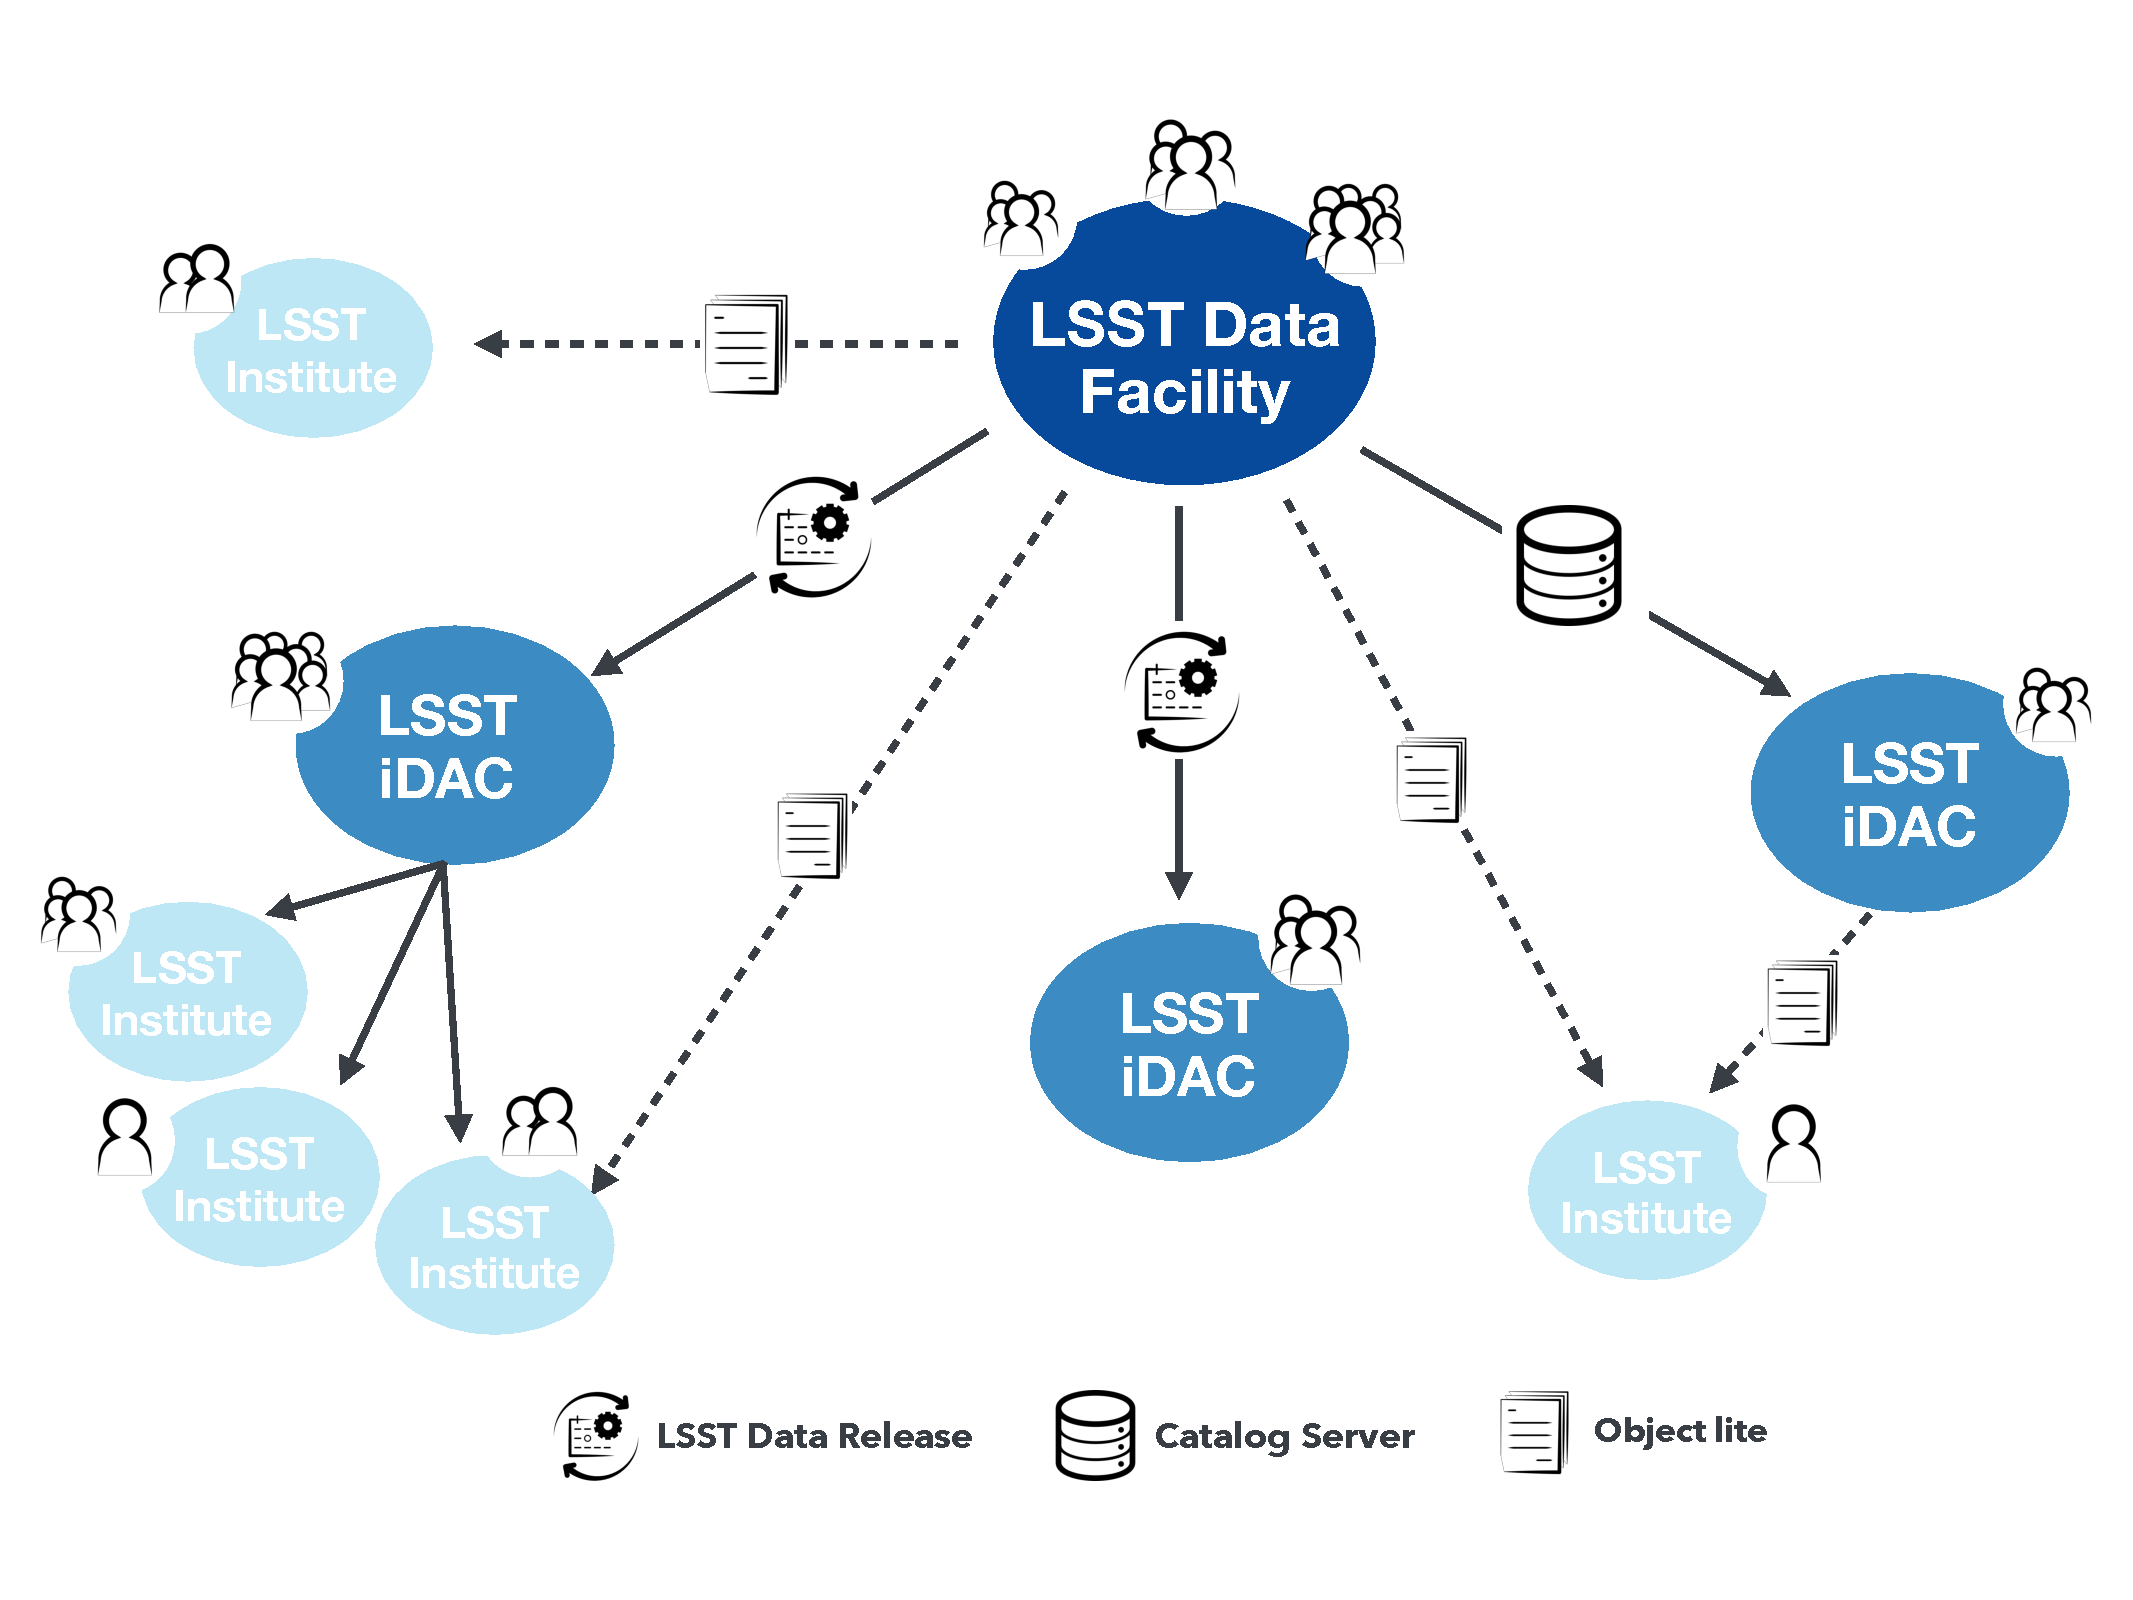
\includegraphics[width=0.8\textwidth]{images_local/LSST-site-topology.pdf}
\caption{LSST Data Facility and Independent DAC network topology.  \label{fig:lsst-site-topology}}
\end{center}
\end{figure}



\subsection{Resources}
{\color{red}Wil } \newline

\subsubsection{Data Storage}
Any institution considering setting up an iDAC will need to show commitment on purchasing sufficient storage and CPU power to hold and serve the data. Sufficient storage ranges from $0.5$ exabytes for the full data release(s) down to $100$ terabytes for a catalog server, and potentially further down to $70$ terabytes if the {\tt Object Lite} option is offered. For the full catalog it is order 100 nodes to serve it up, and to serve images a DAC would need some additional servers; depending on load this may be order 10 additional nodes.

\subsubsection{User Computational}
If the full set of data release products including images and catalogs are desired, it is highly recommended that the iDAC deploy the LSST Science Platform (LSP). The LSP serves as a portal to the data, and provides a user interface of web services and Jupyter notebooks for scientific queries and analysis, an open software framework for astronomy and parallel processing, and the associated computational, storage, and communications infrastructure needed to enable science. The LSP is described in full in \citeds{LSE-319} and \citeds{LDM-554}. Depending on the assumed load, the LSP is relatively modest as it requires only $\sim2$ servers to set up, and it is recommended to have 2 CPUs per simultaneous user (e.g., if the iDAC's desired capability is to serve 200 users, but only expect 50 to be active at a time, then 100 CPUs would be sufficient). From that starting point, the amount of next-to-the-data computational resources can be as large as the data center wishes to provide, and may make use of connecting to e.g., local super computer resources.

\subsubsection{Dedicated Personnel}
The significant hardware required by an iDAC is above the normal level for most astronomy departments, and would require dedicated technical personnel to set it up and keep it running. For an {\tt Object Lite} catalog running on existing hardware, this might not be a significant increase in person power if the hardware is already serving on order $50$--$100$ terabytes. Still, it is recommended to assume $\gtrsim0.25$ full-time equivalent (FTE) personnel hours for {\tt Object Lite}, and perhaps closer to $\sim2$ FTE for the full catalogs, which includes setting up and maintaining the service, and installing new data releases and software updates every year. For iDACs wishing to host the full data releases' images and catalogs and deploy the LSST Science Platform, it becomes necessary to employ $1$--$2$ storage engineers to mange the large amount of data, and possibly one more FTE to keep the Kubernetes (or equivalent) system updated with the latest software deploys. If the iDAC intends to support the science of many local users, support will become a specific issue which may not be covered by the usual institutional funding, and will require further effort. It is therefore recommended that any partner institution wishing to host a full-release iDAC provide a minimum personnel of 5 FTE to be considered viable.

\subsection{Services}
{\color{red} Leanne } \newline

Services provided by LSST partner iDACs:s

\subsubsection{The LSST Science Platform}
All LSST independent data access centres must run an instance of the LSST Science Platform

\subsubsection{User Generated data products }
% Detail here the responsibilities and commitments of the LDF to LSST iDACs. See annex 3.1 

% LPG Outline the responsibilities of the LDF towards recognized iDACs
\section{Responsibilities of the LSST Data Facility} 
{\color{red} Bob } \newline

This section describes the services that the LSST Data Facility (LDF) will provide in support of all LSST iDACs. 

Points to be addressed 
\begin{enumerate}
\item High-bandwidth network out of the LDF to all iDACs
\item Distribution of each of the data products types outlined in \ref{sec:data} to iDACs
\item ......
\end{enumerate}


All LSST  iDACs must be able to serve the 'object-lite' catalog to any institution worldwide. 


\subsection{Proprietary Data Access Policies}
{\color{red}Defer for now until further guidance received.} \newline

All iDACs serving the proprietary LSST data products are subject to the policies in \citeds{LPM-261}. It might be necessary for iDACs to use the LSST authentication system to ensure secure access to the data for authorized users only, and this might require some specific IT work at the iDAC host site.

%%%MLG: commented this out (WOM, delete if we'll never need to say this).
% It remains an open question whether {\em any} qualified user from any LSST partner institution can log into any iDAC -- this would facilitate collaboration but would also require that iDACs participate in the single authentication system.

%%%MLG: commented this out (WOM, delete if we'll never need to say this).
%\subsection{iDACs Serving Post-Proprietary Data}
% {\bf MLG: can we think of any requirements/guidelines for this scenario? Should this document even cover non-partner iDACs? Any non-partner iDAC wishing to serve the two-year-old post-proprietary full release to its users would not, for example, be able to get help installing the LSP. Perhaps we could use this paragraph to further encourage the benefits of partnership.}